\documentclass[twoside]{book}

% Packages required by doxygen
\usepackage{calc}
\usepackage{doxygen}
\usepackage{graphicx}
\usepackage[utf8]{inputenc}
\usepackage{makeidx}
\usepackage{multicol}
\usepackage{multirow}
\usepackage{textcomp}
\usepackage[table]{xcolor}

% NLS support packages
\usepackage{polski}
\usepackage[T1]{fontenc}

% Font selection
\usepackage[T1]{fontenc}
\usepackage{mathptmx}
\usepackage[scaled=.90]{helvet}
\usepackage{courier}
\usepackage{amssymb}
\usepackage{sectsty}
\renewcommand{\familydefault}{\sfdefault}
\allsectionsfont{%
  \fontseries{bc}\selectfont%
  \color{darkgray}%
}
\renewcommand{\DoxyLabelFont}{%
  \fontseries{bc}\selectfont%
  \color{darkgray}%
}

% Page & text layout
\usepackage{geometry}
\geometry{%
  a4paper,%
  top=2.5cm,%
  bottom=2.5cm,%
  left=2.5cm,%
  right=2.5cm%
}
\tolerance=750
\hfuzz=15pt
\hbadness=750
\setlength{\emergencystretch}{15pt}
\setlength{\parindent}{0cm}
\setlength{\parskip}{0.2cm}
\makeatletter
\renewcommand{\paragraph}{%
  \@startsection{paragraph}{4}{0ex}{-1.0ex}{1.0ex}{%
    \normalfont\normalsize\bfseries\SS@parafont%
  }%
}
\renewcommand{\subparagraph}{%
  \@startsection{subparagraph}{5}{0ex}{-1.0ex}{1.0ex}{%
    \normalfont\normalsize\bfseries\SS@subparafont%
  }%
}
\makeatother

% Headers & footers
\usepackage{fancyhdr}
\pagestyle{fancyplain}
\fancyhead[LE]{\fancyplain{}{\bfseries\thepage}}
\fancyhead[CE]{\fancyplain{}{}}
\fancyhead[RE]{\fancyplain{}{\bfseries\leftmark}}
\fancyhead[LO]{\fancyplain{}{\bfseries\rightmark}}
\fancyhead[CO]{\fancyplain{}{}}
\fancyhead[RO]{\fancyplain{}{\bfseries\thepage}}
\fancyfoot[LE]{\fancyplain{}{}}
\fancyfoot[CE]{\fancyplain{}{}}
\fancyfoot[RE]{\fancyplain{}{\bfseries\scriptsize Wygenerowano N, 18 cze 2017 21\-:02\-:49 dla Sense\-Glove programem Doxygen }}
\fancyfoot[LO]{\fancyplain{}{\bfseries\scriptsize Wygenerowano N, 18 cze 2017 21\-:02\-:49 dla Sense\-Glove programem Doxygen }}
\fancyfoot[CO]{\fancyplain{}{}}
\fancyfoot[RO]{\fancyplain{}{}}
\renewcommand{\footrulewidth}{0.4pt}
\renewcommand{\chaptermark}[1]{%
  \markboth{#1}{}%
}
\renewcommand{\sectionmark}[1]{%
  \markright{\thesection\ #1}%
}

% Indices & bibliography
\usepackage{natbib}
\usepackage[titles]{tocloft}
\setcounter{tocdepth}{3}
\setcounter{secnumdepth}{5}
\makeindex

% Hyperlinks (required, but should be loaded last)
\usepackage{ifpdf}
\ifpdf
  \usepackage[pdftex,pagebackref=true]{hyperref}
\else
  \usepackage[ps2pdf,pagebackref=true]{hyperref}
\fi
\hypersetup{%
  colorlinks=true,%
  linkcolor=blue,%
  citecolor=blue,%
  unicode%
}

% Custom commands
\newcommand{\clearemptydoublepage}{%
  \newpage{\pagestyle{empty}\cleardoublepage}%
}


%===== C O N T E N T S =====

\begin{document}

% Titlepage & ToC
\hypersetup{pageanchor=false}
\pagenumbering{roman}
\begin{titlepage}
\vspace*{7cm}
\begin{center}%
{\Large Sense\-Glove \\[1ex]\large 0.\-2.\-3 }\\
\vspace*{1cm}
{\large Wygenerowano przez Doxygen 1.8.6}\\
\vspace*{0.5cm}
{\small N, 18 cze 2017 21:02:49}\\
\end{center}
\end{titlepage}
\clearemptydoublepage
\tableofcontents
\clearemptydoublepage
\pagenumbering{arabic}
\hypersetup{pageanchor=true}

%--- Begin generated contents ---
\chapter{Indeks hierarchiczny}
\section{Hierarchia klas}
Ta lista dziedziczenia posortowana jest z grubsza, choć nie całkowicie, alfabetycznie\+:\begin{DoxyCompactList}
\item Q\+Object\begin{DoxyCompactList}
\item \contentsline{section}{Socket}{\pageref{class_socket}}{}
\end{DoxyCompactList}
\item Q\+Thread\begin{DoxyCompactList}
\item \contentsline{section}{Read\+\_\+\+Thread}{\pageref{class_read___thread}}{}
\end{DoxyCompactList}
\item Q\+Widget\begin{DoxyCompactList}
\item \contentsline{section}{Okno}{\pageref{class_okno}}{}
\end{DoxyCompactList}
\end{DoxyCompactList}

\chapter{Indeks klas}
\section{Lista klas}
Tutaj znajdują się klasy, struktury, unie i interfejsy wraz z ich krótkimi opisami\+:\begin{DoxyCompactList}
\item\contentsline{section}{\hyperlink{class_okno}{Okno} \\*The \hyperlink{class_okno}{Okno} class okno główne programu }{\pageref{class_okno}}{}
\item\contentsline{section}{\hyperlink{class_read___thread}{Read\+\_\+\+Thread} \\*The \hyperlink{class_read___thread}{Read\+\_\+\+Thread} class watek czytajacy z portu U\+SB }{\pageref{class_read___thread}}{}
\item\contentsline{section}{\hyperlink{class_socket}{Socket} \\*The \hyperlink{class_socket}{Socket} class }{\pageref{class_socket}}{}
\end{DoxyCompactList}

\chapter{Dokumentacja klas}
\hypertarget{class_okno}{\section{Dokumentacja klasy Okno}
\label{class_okno}\index{Okno@{Okno}}
}


The \hyperlink{class_okno}{Okno} class \hyperlink{class_okno}{Okno} główne programu.  




{\ttfamily \#include $<$okno.\-hh$>$}

Diagram dziedziczenia dla Okno\begin{figure}[H]
\begin{center}
\leavevmode
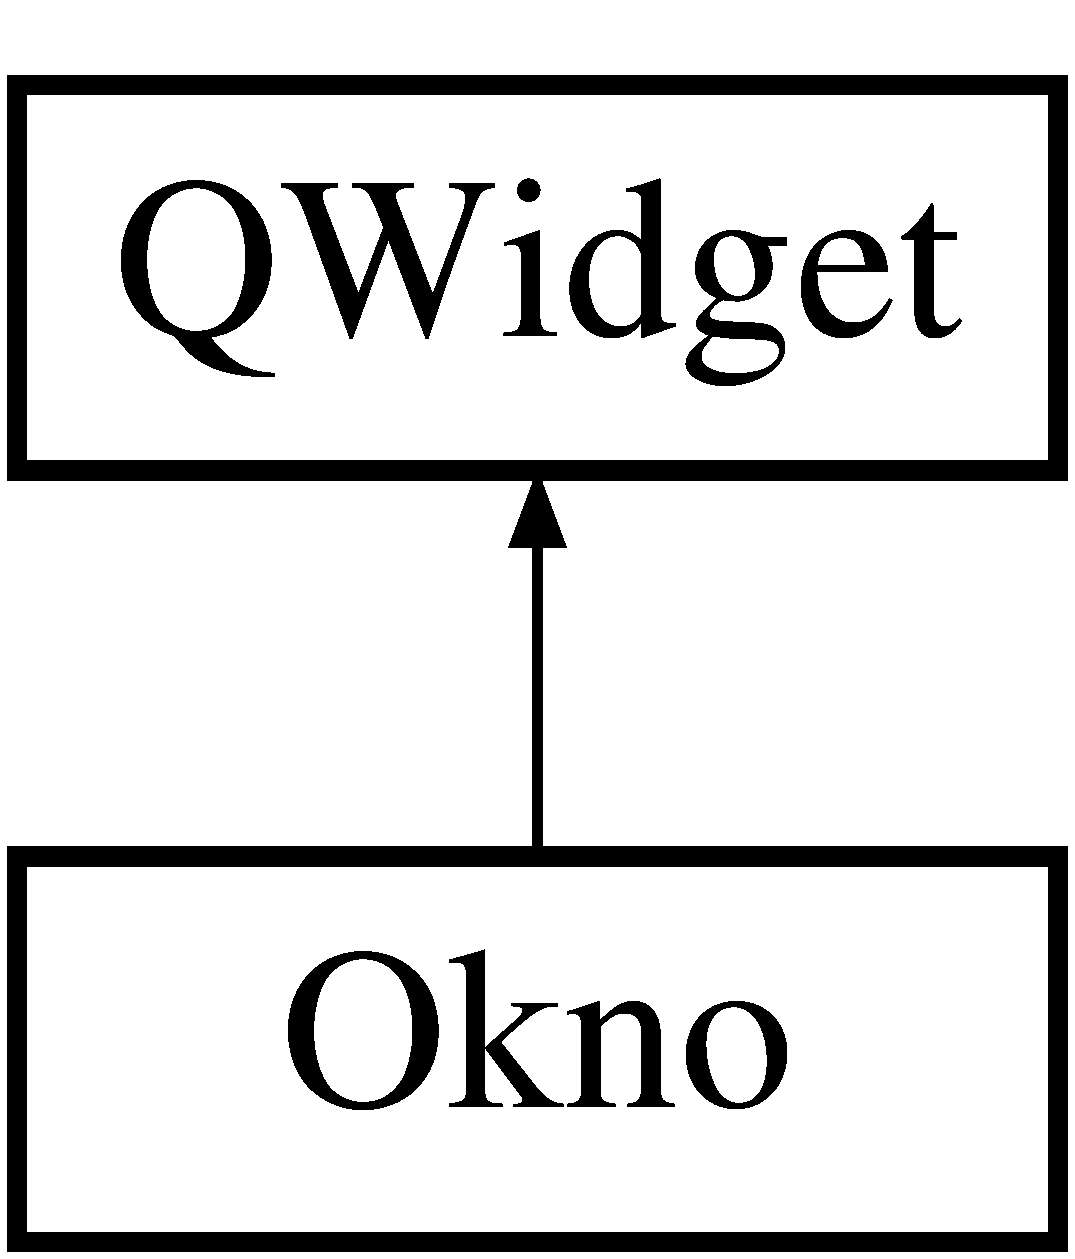
\includegraphics[height=2.000000cm]{class_okno}
\end{center}
\end{figure}
\subsection*{Sloty publiczne}
\begin{DoxyCompactItemize}
\item 
\hypertarget{class_okno_ad6a171a82ec052ba0e8c721ffac0e870}{void \hyperlink{class_okno_ad6a171a82ec052ba0e8c721ffac0e870}{on\-\_\-start\-\_\-clicked} ()}\label{class_okno_ad6a171a82ec052ba0e8c721ffac0e870}

\begin{DoxyCompactList}\small\item\em \hyperlink{class_okno_ad6a171a82ec052ba0e8c721ffac0e870}{Okno\-::on\-\_\-start\-\_\-clicked} Rozpoczęcie wątku odczytującego dane, sprawdzenie poprawności otwarcia wybranego portu U\-S\-B, możliwość ponownego wyboru portu U\-S\-B. \end{DoxyCompactList}\item 
\hypertarget{class_okno_ad3e545f9470f154d09ab9cf91bee0b2a}{void \hyperlink{class_okno_ad3e545f9470f154d09ab9cf91bee0b2a}{on\-\_\-start\-\_\-m\-\_\-clicked} ()}\label{class_okno_ad3e545f9470f154d09ab9cf91bee0b2a}

\begin{DoxyCompactList}\small\item\em \hyperlink{class_okno_ad3e545f9470f154d09ab9cf91bee0b2a}{Okno\-::on\-\_\-start\-\_\-m\-\_\-clicked} Uruchomienie pomiaru, ustawienie odpowiednich przycisków, uruchomienie timerów. \end{DoxyCompactList}\item 
\hypertarget{class_okno_ae30bfa2ba063af6dac4680291bccb6cd}{void \hyperlink{class_okno_ae30bfa2ba063af6dac4680291bccb6cd}{Set\-Progress\-Bar} ()}\label{class_okno_ae30bfa2ba063af6dac4680291bccb6cd}

\begin{DoxyCompactList}\small\item\em Set\-Progress\-Bar zwiekszanie wartosci progress\-\_\-bar poloczone z sygnalem z timera bartim. \end{DoxyCompactList}\item 
\hypertarget{class_okno_aaf9c12bca53a881c5492cd7779cdecad}{void \hyperlink{class_okno_aaf9c12bca53a881c5492cd7779cdecad}{set\-Measure\-Icons} ()}\label{class_okno_aaf9c12bca53a881c5492cd7779cdecad}

\begin{DoxyCompactList}\small\item\em \hyperlink{class_okno_aaf9c12bca53a881c5492cd7779cdecad}{Okno\-::set\-Measure\-Icons} Public slot połaczony z sygnałem z timera, który odmierza 2s na pomiar. \end{DoxyCompactList}\item 
\hypertarget{class_okno_a6fea95038d5967dd336b87935b97170c}{void \hyperlink{class_okno_a6fea95038d5967dd336b87935b97170c}{on\-\_\-accept\-\_\-clicked} ()}\label{class_okno_a6fea95038d5967dd336b87935b97170c}

\begin{DoxyCompactList}\small\item\em \hyperlink{class_okno_a6fea95038d5967dd336b87935b97170c}{Okno\-::on\-\_\-accept\-\_\-clicked} Uruchamia zapisywanie do pliku danych z tablicy data\mbox{[}\mbox{]}. \end{DoxyCompactList}\item 
\hypertarget{class_okno_a15073474701e4bec563b6a2cdad11ac4}{void \hyperlink{class_okno_a15073474701e4bec563b6a2cdad11ac4}{on\-\_\-reject\-\_\-clicked} ()}\label{class_okno_a15073474701e4bec563b6a2cdad11ac4}

\begin{DoxyCompactList}\small\item\em \hyperlink{class_okno_a15073474701e4bec563b6a2cdad11ac4}{Okno\-::on\-\_\-reject\-\_\-clicked} Ignoruje dane zapisane do tablicy, powoduje pojawienie się odpowiednich przycisków. \end{DoxyCompactList}\end{DoxyCompactItemize}
\subsection*{Metody publiczne}
\begin{DoxyCompactItemize}
\item 
\hyperlink{class_okno_ab0e6342aaa2ff2cd07598a901528efa6}{Okno} (Q\-Widget $\ast$parent)
\begin{DoxyCompactList}\small\item\em \hyperlink{class_okno_ab0e6342aaa2ff2cd07598a901528efa6}{Okno\-::\-Okno}. \end{DoxyCompactList}\item 
void \hyperlink{class_okno_a20d42ba81a2b4b83bed90cb1dc687362}{set\-Desk\-Port} (int Desk\-Portu)
\begin{DoxyCompactList}\small\item\em set\-Desk\-Port \end{DoxyCompactList}\item 
int \hyperlink{class_okno_a3d917a01365c453f29c8f8ff78cd67b7}{take\-Desk\-Port} () const 
\begin{DoxyCompactList}\small\item\em take\-Desk\-Port \end{DoxyCompactList}\item 
\hypertarget{class_okno_acb4f4dd5dfc929b4e019c1c169c9df0c}{void \hyperlink{class_okno_acb4f4dd5dfc929b4e019c1c169c9df0c}{end\-Read\-Thread} ()}\label{class_okno_acb4f4dd5dfc929b4e019c1c169c9df0c}

\begin{DoxyCompactList}\small\item\em end\-Read\-Thread konczenie watku czytajacego z U\-S\-B \end{DoxyCompactList}\item 
\hypertarget{class_okno_a8f6f59862bff738dbf5f650274fb1058}{void \hyperlink{class_okno_a8f6f59862bff738dbf5f650274fb1058}{wait\-Read\-Thread} ()}\label{class_okno_a8f6f59862bff738dbf5f650274fb1058}

\begin{DoxyCompactList}\small\item\em wait\-Read\-Thread czekanie na zakonczenie watku \end{DoxyCompactList}\item 
bool \hyperlink{class_okno_a24f3d0d347964d7da0cde1929ab23c41}{Save\-To\-File} ()
\begin{DoxyCompactList}\small\item\em \hyperlink{class_okno_a24f3d0d347964d7da0cde1929ab23c41}{Okno\-::\-Save\-To\-File} Zapisywanie do pliku z tablicy data\mbox{[}\mbox{]}. Rozdzielenie danych na poszczególne czujniki. \end{DoxyCompactList}\end{DoxyCompactItemize}
\subsection*{Atrybuty publiczne}
\begin{DoxyCompactItemize}
\item 
\hypertarget{class_okno_a0cd2b4f8ec74806cc7d3256eff69385a}{bool \hyperlink{class_okno_a0cd2b4f8ec74806cc7d3256eff69385a}{start\-\_\-flag}}\label{class_okno_a0cd2b4f8ec74806cc7d3256eff69385a}

\begin{DoxyCompactList}\small\item\em start\-\_\-flag -\/ flaga oznaczająca początek czytanai wątku \end{DoxyCompactList}\item 
\hypertarget{class_okno_ac9c31fbce4cb68413088827860277510}{int \hyperlink{class_okno_ac9c31fbce4cb68413088827860277510}{desk\-\_\-portu}}\label{class_okno_ac9c31fbce4cb68413088827860277510}

\begin{DoxyCompactList}\small\item\em desk\-\_\-portu \end{DoxyCompactList}\item 
\hypertarget{class_okno_a5a94843afcfc67735c25e5a29f9cdc3c}{bool \hyperlink{class_okno_a5a94843afcfc67735c25e5a29f9cdc3c}{measure\-\_\-flag}}\label{class_okno_a5a94843afcfc67735c25e5a29f9cdc3c}

\begin{DoxyCompactList}\small\item\em measure\-\_\-flag \end{DoxyCompactList}\item 
\hypertarget{class_okno_afddfe7d21fc34910d75f92d8904acb23}{bool \hyperlink{class_okno_afddfe7d21fc34910d75f92d8904acb23}{save\-\_\-flag}}\label{class_okno_afddfe7d21fc34910d75f92d8904acb23}

\begin{DoxyCompactList}\small\item\em save\-\_\-flag \end{DoxyCompactList}\item 
\hypertarget{class_okno_a6f836849c2547fcb51936a9c88c8e75a}{\hyperlink{class_read___thread}{Read\-\_\-\-Thread} \hyperlink{class_okno_a6f836849c2547fcb51936a9c88c8e75a}{read\-\_\-thread}}\label{class_okno_a6f836849c2547fcb51936a9c88c8e75a}

\begin{DoxyCompactList}\small\item\em read\-\_\-thread \end{DoxyCompactList}\item 
\hypertarget{class_okno_af210b4fcf0872b832f3cc49bace1c48d}{Q\-Vector$<$ string $>$ \hyperlink{class_okno_af210b4fcf0872b832f3cc49bace1c48d}{data}}\label{class_okno_af210b4fcf0872b832f3cc49bace1c48d}

\begin{DoxyCompactList}\small\item\em data -\/ dane do przesyłu poprzez socket \end{DoxyCompactList}\item 
\hypertarget{class_okno_a58a686222d1cc92f47d454c2481ce8d8}{\hyperlink{class_socket}{Socket} $\ast$ \hyperlink{class_okno_a58a686222d1cc92f47d454c2481ce8d8}{my\-Socket}}\label{class_okno_a58a686222d1cc92f47d454c2481ce8d8}

\begin{DoxyCompactList}\small\item\em my\-Socket -\/ socket, przez który wysyłane są dane \end{DoxyCompactList}\end{DoxyCompactItemize}
\subsection*{Metody chronione}
\begin{DoxyCompactItemize}
\item 
void \hyperlink{class_okno_aecd3efa2e5687dad240bf830c73984ba}{close\-Event} (Q\-Close\-Event $\ast$clevent)
\begin{DoxyCompactList}\small\item\em \hyperlink{class_okno_aecd3efa2e5687dad240bf830c73984ba}{Okno\-::close\-Event}. \end{DoxyCompactList}\end{DoxyCompactItemize}
\subsection*{Atrybuty prywatne}
\begin{DoxyCompactItemize}
\item 
\hypertarget{class_okno_a0ca5cf439ed8ad3ab7ef7b854c267f1b}{Q\-Timer $\ast$ \hyperlink{class_okno_a0ca5cf439ed8ad3ab7ef7b854c267f1b}{timer}}\label{class_okno_a0ca5cf439ed8ad3ab7ef7b854c267f1b}

\begin{DoxyCompactList}\small\item\em timer Timer służący do odmierzania 2 s pomiaru. \end{DoxyCompactList}\item 
\hypertarget{class_okno_a0c69b007d741152d74b5d3d498289a48}{Q\-Timer $\ast$ \hyperlink{class_okno_a0c69b007d741152d74b5d3d498289a48}{bartim}}\label{class_okno_a0c69b007d741152d74b5d3d498289a48}

\begin{DoxyCompactList}\small\item\em bartim Timer odmierzający czas dla paska ładowania. \end{DoxyCompactList}\item 
\hypertarget{class_okno_aebc2e861da784f50f7965b17cfd8a85e}{Q\-Progress\-Bar $\ast$ \hyperlink{class_okno_aebc2e861da784f50f7965b17cfd8a85e}{progress\-\_\-bar}}\label{class_okno_aebc2e861da784f50f7965b17cfd8a85e}

\begin{DoxyCompactList}\small\item\em progress\-\_\-bar Pasek ładowania pokazujący postęp pomiaru danych. \end{DoxyCompactList}\item 
\hypertarget{class_okno_a69cde4a1b1adcb98dd0f74b4a27a13e8}{Q\-Label $\ast$ \hyperlink{class_okno_a69cde4a1b1adcb98dd0f74b4a27a13e8}{usb\-\_\-label}}\label{class_okno_a69cde4a1b1adcb98dd0f74b4a27a13e8}

\begin{DoxyCompactList}\small\item\em usb\-\_\-label Napis z informacją o możliwości wyboru portu U\-S\-B. \end{DoxyCompactList}\item 
\hypertarget{class_okno_ae069d59c53771223e2c82d6d6ace45d3}{Q\-Combo\-Box $\ast$ \hyperlink{class_okno_ae069d59c53771223e2c82d6d6ace45d3}{usb\-\_\-choice}}\label{class_okno_ae069d59c53771223e2c82d6d6ace45d3}

\begin{DoxyCompactList}\small\item\em usb\-\_\-choice Lista wyboru portu U\-S\-B. \end{DoxyCompactList}\item 
\hypertarget{class_okno_ae7cda77331e084b73b3065c4cc5e46d2}{Q\-Push\-Button $\ast$ \hyperlink{class_okno_ae7cda77331e084b73b3065c4cc5e46d2}{start}}\label{class_okno_ae7cda77331e084b73b3065c4cc5e46d2}

\begin{DoxyCompactList}\small\item\em start Przycisk startu przesyłania danych do programu wizualizacji. \end{DoxyCompactList}\item 
\hypertarget{class_okno_a211a0bea332494946d0417ebb6c73ae3}{Q\-Push\-Button $\ast$ \hyperlink{class_okno_a211a0bea332494946d0417ebb6c73ae3}{start\-\_\-m}}\label{class_okno_a211a0bea332494946d0417ebb6c73ae3}

\begin{DoxyCompactList}\small\item\em start\-\_\-m Przycisk startu pomiaru. \end{DoxyCompactList}\item 
\hypertarget{class_okno_a4fe774bd293a9dd438b803279b1cdd3a}{Q\-Push\-Button $\ast$ \hyperlink{class_okno_a4fe774bd293a9dd438b803279b1cdd3a}{accept}}\label{class_okno_a4fe774bd293a9dd438b803279b1cdd3a}

\begin{DoxyCompactList}\small\item\em accept Przycisk akceptacji pomiaru. \end{DoxyCompactList}\item 
\hypertarget{class_okno_a70bd37b785ed16ce6db16f5b434ab75a}{Q\-Push\-Button $\ast$ \hyperlink{class_okno_a70bd37b785ed16ce6db16f5b434ab75a}{reject}}\label{class_okno_a70bd37b785ed16ce6db16f5b434ab75a}

\begin{DoxyCompactList}\small\item\em reject Przycisk odrzucenia pomiaru. \end{DoxyCompactList}\item 
\hypertarget{class_okno_a00ebd56e108eee1419ef68f9f68bfce3}{Q\-Grid\-Layout $\ast$ \hyperlink{class_okno_a00ebd56e108eee1419ef68f9f68bfce3}{layout}}\label{class_okno_a00ebd56e108eee1419ef68f9f68bfce3}

\begin{DoxyCompactList}\small\item\em layout Warstwa potrzebna do ustawienia wzgledem siebie elementów. \end{DoxyCompactList}\item 
\hypertarget{class_okno_aba409a1e85e08d5f5f0dea2ae784dd18}{Q\-Combo\-Box $\ast$ \hyperlink{class_okno_aba409a1e85e08d5f5f0dea2ae784dd18}{type\-\_\-of\-\_\-movement}}\label{class_okno_aba409a1e85e08d5f5f0dea2ae784dd18}

\begin{DoxyCompactList}\small\item\em type\-\_\-of\-\_\-movement Lista wyboru typu ruchu. \end{DoxyCompactList}\item 
\hypertarget{class_okno_add48fe820613017f93c66278e8b648de}{Q\-Label $\ast$ \hyperlink{class_okno_add48fe820613017f93c66278e8b648de}{name\-\_\-label}}\label{class_okno_add48fe820613017f93c66278e8b648de}

\begin{DoxyCompactList}\small\item\em name\-\_\-label Napis informujący o możliwości podania imienia osoby wykonującej pomiar. \end{DoxyCompactList}\item 
\hypertarget{class_okno_ad86ed0c15931f5567519da354b9fb1e4}{Q\-Line\-Edit $\ast$ \hyperlink{class_okno_ad86ed0c15931f5567519da354b9fb1e4}{name}}\label{class_okno_ad86ed0c15931f5567519da354b9fb1e4}

\begin{DoxyCompactList}\small\item\em name Pole do podania imienia osoby wykonujacej pomiar. \end{DoxyCompactList}\item 
\hypertarget{class_okno_a0f42040af518729eb012f77f2f4b2f6e}{Q\-Label $\ast$ \hyperlink{class_okno_a0f42040af518729eb012f77f2f4b2f6e}{move\-\_\-name}}\label{class_okno_a0f42040af518729eb012f77f2f4b2f6e}

\begin{DoxyCompactList}\small\item\em move\-\_\-name Napis informujacy o rodzaju wykonanego ruchu. \end{DoxyCompactList}\end{DoxyCompactItemize}


\subsection{Opis szczegółowy}
The \hyperlink{class_okno}{Okno} class \hyperlink{class_okno}{Okno} główne programu. 

\subsection{Dokumentacja konstruktora i destruktora}
\hypertarget{class_okno_ab0e6342aaa2ff2cd07598a901528efa6}{\index{Okno@{Okno}!Okno@{Okno}}
\index{Okno@{Okno}!Okno@{Okno}}
\subsubsection[{Okno}]{\setlength{\rightskip}{0pt plus 5cm}Okno\-::\-Okno (
\begin{DoxyParamCaption}
\item[{Q\-Widget $\ast$}]{parent}
\end{DoxyParamCaption}
)}}\label{class_okno_ab0e6342aaa2ff2cd07598a901528efa6}


\hyperlink{class_okno_ab0e6342aaa2ff2cd07598a901528efa6}{Okno\-::\-Okno}. 


\begin{DoxyParams}{Parametry}
{\em parent} & Konstruktor okna głównego programu, inicjalizacja wszystkich parametrów. \\
\hline
\end{DoxyParams}


\subsection{Dokumentacja funkcji składowych}
\hypertarget{class_okno_aecd3efa2e5687dad240bf830c73984ba}{\index{Okno@{Okno}!close\-Event@{close\-Event}}
\index{close\-Event@{close\-Event}!Okno@{Okno}}
\subsubsection[{close\-Event}]{\setlength{\rightskip}{0pt plus 5cm}void Okno\-::close\-Event (
\begin{DoxyParamCaption}
\item[{Q\-Close\-Event $\ast$}]{clevent}
\end{DoxyParamCaption}
)\hspace{0.3cm}{\ttfamily [protected]}}}\label{class_okno_aecd3efa2e5687dad240bf830c73984ba}


\hyperlink{class_okno_aecd3efa2e5687dad240bf830c73984ba}{Okno\-::close\-Event}. 

Zamknięcie wątku read\-\_\-thread. \hypertarget{class_okno_a24f3d0d347964d7da0cde1929ab23c41}{\index{Okno@{Okno}!Save\-To\-File@{Save\-To\-File}}
\index{Save\-To\-File@{Save\-To\-File}!Okno@{Okno}}
\subsubsection[{Save\-To\-File}]{\setlength{\rightskip}{0pt plus 5cm}bool Okno\-::\-Save\-To\-File (
\begin{DoxyParamCaption}
{}
\end{DoxyParamCaption}
)}}\label{class_okno_a24f3d0d347964d7da0cde1929ab23c41}


\hyperlink{class_okno_a24f3d0d347964d7da0cde1929ab23c41}{Okno\-::\-Save\-To\-File} Zapisywanie do pliku z tablicy data\mbox{[}\mbox{]}. Rozdzielenie danych na poszczególne czujniki. 

\begin{DoxyReturn}{Zwraca}
bool -\/ czy zapis do pliku się powiodl czy nie 
\end{DoxyReturn}
\hypertarget{class_okno_a20d42ba81a2b4b83bed90cb1dc687362}{\index{Okno@{Okno}!set\-Desk\-Port@{set\-Desk\-Port}}
\index{set\-Desk\-Port@{set\-Desk\-Port}!Okno@{Okno}}
\subsubsection[{set\-Desk\-Port}]{\setlength{\rightskip}{0pt plus 5cm}void Okno\-::set\-Desk\-Port (
\begin{DoxyParamCaption}
\item[{int}]{Desk\-Portu}
\end{DoxyParamCaption}
)\hspace{0.3cm}{\ttfamily [inline]}}}\label{class_okno_a20d42ba81a2b4b83bed90cb1dc687362}


set\-Desk\-Port 


\begin{DoxyParams}{Parametry}
{\em Desk\-Portu} & \\
\hline
\end{DoxyParams}
\hypertarget{class_okno_a3d917a01365c453f29c8f8ff78cd67b7}{\index{Okno@{Okno}!take\-Desk\-Port@{take\-Desk\-Port}}
\index{take\-Desk\-Port@{take\-Desk\-Port}!Okno@{Okno}}
\subsubsection[{take\-Desk\-Port}]{\setlength{\rightskip}{0pt plus 5cm}int Okno\-::take\-Desk\-Port (
\begin{DoxyParamCaption}
{}
\end{DoxyParamCaption}
) const\hspace{0.3cm}{\ttfamily [inline]}}}\label{class_okno_a3d917a01365c453f29c8f8ff78cd67b7}


take\-Desk\-Port 

\begin{DoxyReturn}{Zwraca}
zwraca desk\-\_\-portu 
\end{DoxyReturn}


Dokumentacja dla tej klasy została wygenerowana z plików\-:\begin{DoxyCompactItemize}
\item 
/home/tofik/\-S\-G/data\-\_\-acquisition/prj/inc/okno.\-hh\item 
/home/tofik/\-S\-G/data\-\_\-acquisition/prj/src/okno.\-cpp\end{DoxyCompactItemize}

\hypertarget{class_read___thread}{}\section{Dokumentacja klasy Read\+\_\+\+Thread}
\label{class_read___thread}\index{Read\+\_\+\+Thread@{Read\+\_\+\+Thread}}


The \hyperlink{class_read___thread}{Read\+\_\+\+Thread} class watek czytajacy z portu U\+SB.  




{\ttfamily \#include $<$okno.\+hh$>$}

Diagram dziedziczenia dla Read\+\_\+\+Thread\begin{figure}[H]
\begin{center}
\leavevmode
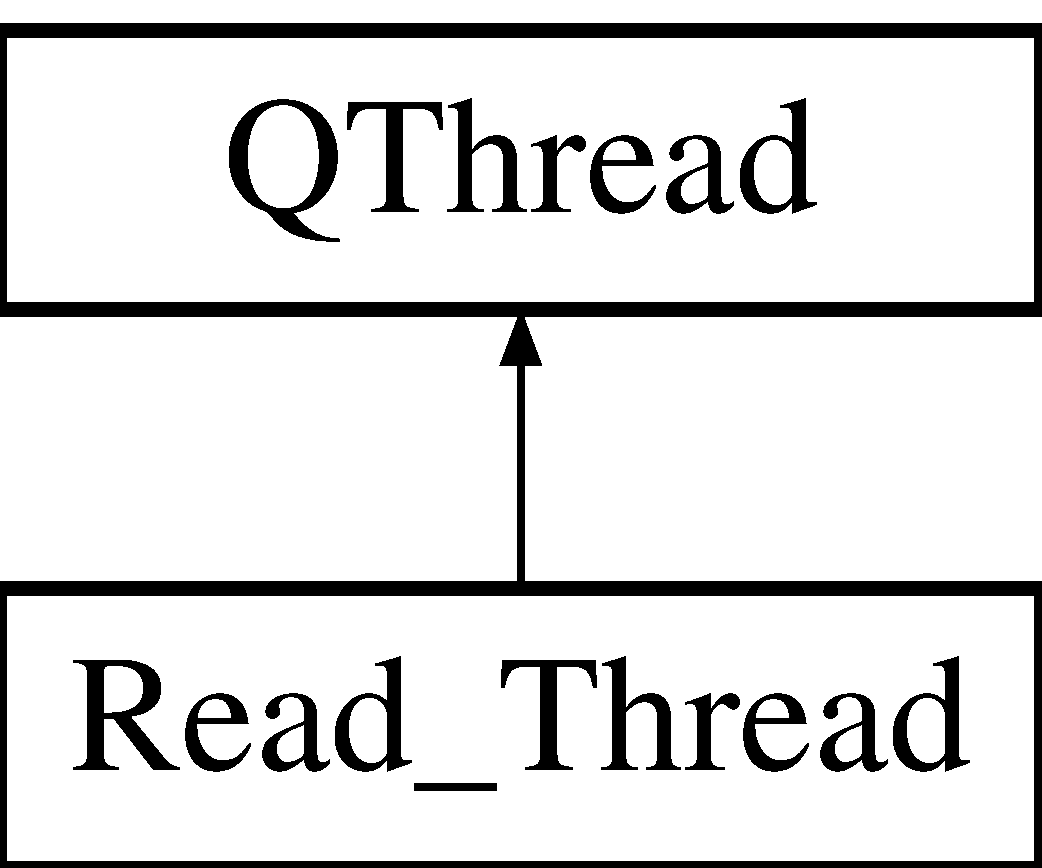
\includegraphics[height=2.000000cm]{class_read___thread}
\end{center}
\end{figure}
\subsection*{Metody publiczne}
\begin{DoxyCompactItemize}
\item 
\hyperlink{class_read___thread_a75267b0bd2c0061ff8998a51470de609}{Read\+\_\+\+Thread} (Q\+Object $\ast$parent, \hyperlink{class_okno}{Okno} $\ast$\+\_\+window)
\begin{DoxyCompactList}\small\item\em \hyperlink{class_read___thread}{Read\+\_\+\+Thread}. \end{DoxyCompactList}\item 
void \hyperlink{class_read___thread_aac135df28f316466b880187097a268fd}{Start} ()\hypertarget{class_read___thread_aac135df28f316466b880187097a268fd}{}\label{class_read___thread_aac135df28f316466b880187097a268fd}

\begin{DoxyCompactList}\small\item\em Start -\/ funkcja zaczynjąca wątek i ustawiająca mu start\+\_\+flag=true. \end{DoxyCompactList}\item 
void \hyperlink{class_read___thread_ab7f432f2160c3e884af7a80387764977}{Stop} ()\hypertarget{class_read___thread_ab7f432f2160c3e884af7a80387764977}{}\label{class_read___thread_ab7f432f2160c3e884af7a80387764977}

\begin{DoxyCompactList}\small\item\em Stop -\/ funkcja ustawiająca start\+\_\+flag=false. \end{DoxyCompactList}\item 
void \hyperlink{class_read___thread_a261a3cc9c3dc6abe61946123c3de76dc}{run} ()
\begin{DoxyCompactList}\small\item\em \hyperlink{class_read___thread_a261a3cc9c3dc6abe61946123c3de76dc}{Read\+\_\+\+Thread\+::run}. \end{DoxyCompactList}\item 
bool \hyperlink{class_read___thread_a4b81499a6d426573733446d4af8e7b07}{Check\+Data} (Q\+String $\ast$wiadomosc)
\begin{DoxyCompactList}\small\item\em \hyperlink{class_read___thread_a4b81499a6d426573733446d4af8e7b07}{Read\+\_\+\+Thread\+::\+Check\+Data} Sprawdzanie sumy kontrolnej, suma wartości z wszystkich czujnikow modulo 2$^\wedge$16. \end{DoxyCompactList}\end{DoxyCompactItemize}
\subsection*{Atrybuty prywatne}
\begin{DoxyCompactItemize}
\item 
\hyperlink{class_okno}{Okno} $\ast$ {\bfseries window}\hypertarget{class_read___thread_a0c9db3caef6b98a0528dc2995801d4bd}{}\label{class_read___thread_a0c9db3caef6b98a0528dc2995801d4bd}

\item 
bool {\bfseries start\+\_\+flag}\hypertarget{class_read___thread_ac79ca6e83cd0246d67b2fd0a5e0c2c2c}{}\label{class_read___thread_ac79ca6e83cd0246d67b2fd0a5e0c2c2c}

\end{DoxyCompactItemize}


\subsection{Opis szczegółowy}
The \hyperlink{class_read___thread}{Read\+\_\+\+Thread} class watek czytajacy z portu U\+SB. 

\subsection{Dokumentacja konstruktora i destruktora}
\index{Read\+\_\+\+Thread@{Read\+\_\+\+Thread}!Read\+\_\+\+Thread@{Read\+\_\+\+Thread}}
\index{Read\+\_\+\+Thread@{Read\+\_\+\+Thread}!Read\+\_\+\+Thread@{Read\+\_\+\+Thread}}
\subsubsection[{\texorpdfstring{Read\+\_\+\+Thread(\+Q\+Object $\ast$parent, Okno $\ast$\+\_\+window)}{Read_Thread(QObject *parent, Okno *_window)}}]{\setlength{\rightskip}{0pt plus 5cm}Read\+\_\+\+Thread\+::\+Read\+\_\+\+Thread (
\begin{DoxyParamCaption}
\item[{Q\+Object $\ast$}]{parent, }
\item[{{\bf Okno} $\ast$}]{\+\_\+window}
\end{DoxyParamCaption}
)\hspace{0.3cm}{\ttfamily [inline]}}\hypertarget{class_read___thread_a75267b0bd2c0061ff8998a51470de609}{}\label{class_read___thread_a75267b0bd2c0061ff8998a51470de609}


\hyperlink{class_read___thread}{Read\+\_\+\+Thread}. 


\begin{DoxyParams}{Parametry}
{\em parent} & \\
\hline
{\em \+\_\+window} & konstruktor watku \\
\hline
\end{DoxyParams}


\subsection{Dokumentacja funkcji składowych}
\index{Read\+\_\+\+Thread@{Read\+\_\+\+Thread}!Check\+Data@{Check\+Data}}
\index{Check\+Data@{Check\+Data}!Read\+\_\+\+Thread@{Read\+\_\+\+Thread}}
\subsubsection[{\texorpdfstring{Check\+Data(\+Q\+String $\ast$wiadomosc)}{CheckData(QString *wiadomosc)}}]{\setlength{\rightskip}{0pt plus 5cm}bool Read\+\_\+\+Thread\+::\+Check\+Data (
\begin{DoxyParamCaption}
\item[{Q\+String $\ast$}]{wiadomosc}
\end{DoxyParamCaption}
)}\hypertarget{class_read___thread_a4b81499a6d426573733446d4af8e7b07}{}\label{class_read___thread_a4b81499a6d426573733446d4af8e7b07}


\hyperlink{class_read___thread_a4b81499a6d426573733446d4af8e7b07}{Read\+\_\+\+Thread\+::\+Check\+Data} Sprawdzanie sumy kontrolnej, suma wartości z wszystkich czujnikow modulo 2$^\wedge$16. 


\begin{DoxyParams}{Parametry}
{\em wiadomosc} & -\/\\
\hline
\end{DoxyParams}
\begin{DoxyReturn}{Zwraca}
true -\/ dane poprawne, false -\/ dane niepoprawne 
\end{DoxyReturn}
\index{Read\+\_\+\+Thread@{Read\+\_\+\+Thread}!run@{run}}
\index{run@{run}!Read\+\_\+\+Thread@{Read\+\_\+\+Thread}}
\subsubsection[{\texorpdfstring{run()}{run()}}]{\setlength{\rightskip}{0pt plus 5cm}void Read\+\_\+\+Thread\+::run (
\begin{DoxyParamCaption}
{}
\end{DoxyParamCaption}
)}\hypertarget{class_read___thread_a261a3cc9c3dc6abe61946123c3de76dc}{}\label{class_read___thread_a261a3cc9c3dc6abe61946123c3de76dc}


\hyperlink{class_read___thread_a261a3cc9c3dc6abe61946123c3de76dc}{Read\+\_\+\+Thread\+::run}. 

Watek czytajacy z portu U\+SB W razie ustawienie odpowiednich flag zapisuje też dane do tablicy data\mbox{[}\mbox{]} 

Dokumentacja dla tej klasy została wygenerowana z plików\+:\begin{DoxyCompactItemize}
\item 
/home/ad/\+S\+E\+N\+S\+G\+L\+O\+V\+E/\+S\+G/data\+\_\+acquisition/prj/inc/okno.\+hh\item 
/home/ad/\+S\+E\+N\+S\+G\+L\+O\+V\+E/\+S\+G/data\+\_\+acquisition/prj/src/okno.\+cpp\end{DoxyCompactItemize}

\hypertarget{class_socket}{}\section{Dokumentacja klasy Socket}
\label{class_socket}\index{Socket@{Socket}}


The \hyperlink{class_socket}{Socket} class.  




{\ttfamily \#include $<$socket.\+hh$>$}

Diagram dziedziczenia dla Socket\begin{figure}[H]
\begin{center}
\leavevmode
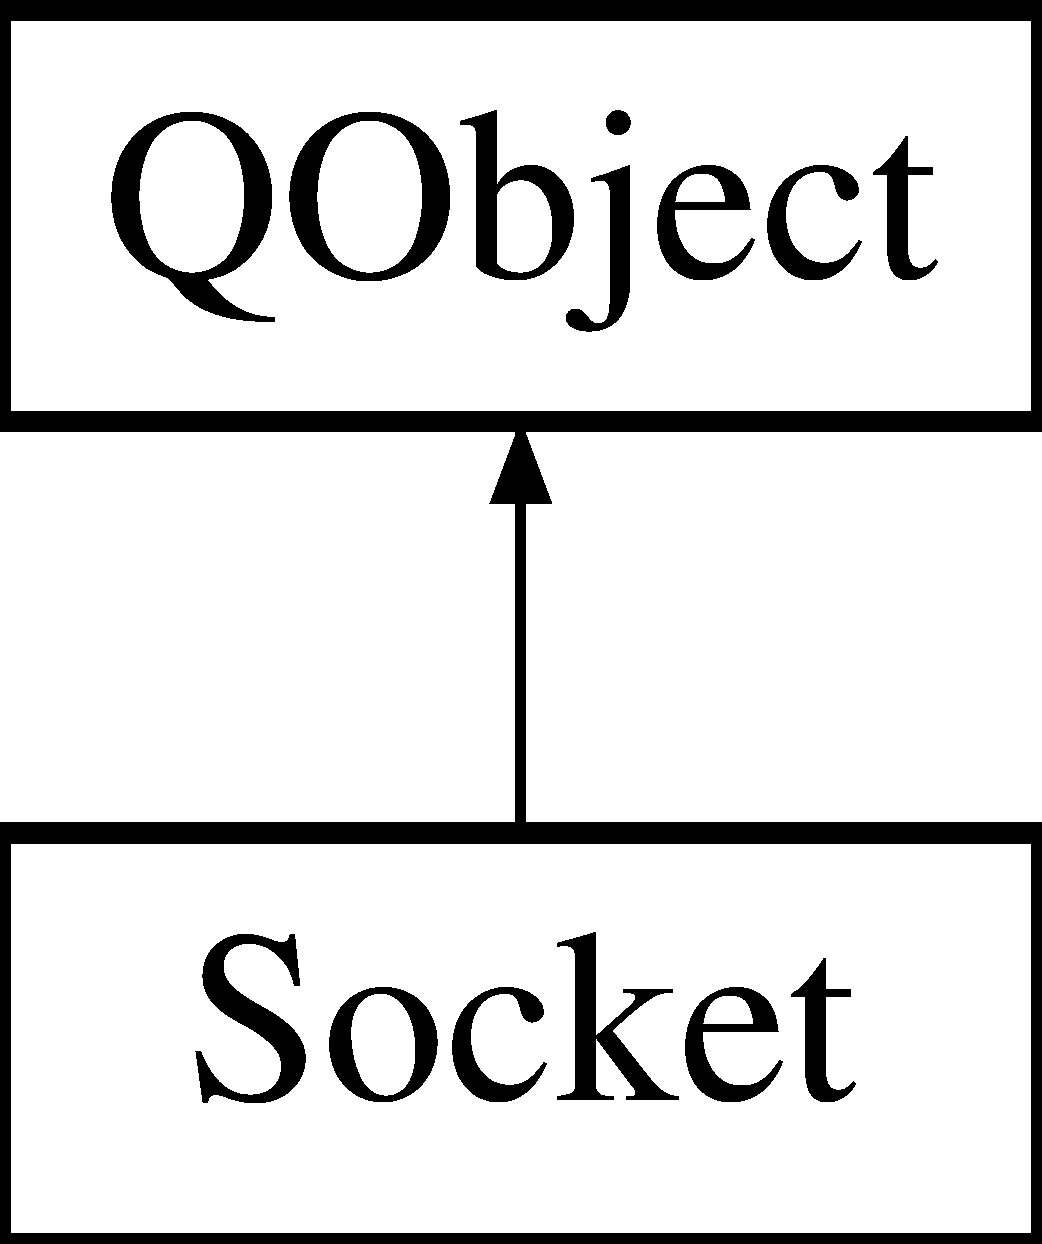
\includegraphics[height=2.000000cm]{class_socket}
\end{center}
\end{figure}
\subsection*{Sloty publiczne}
\begin{DoxyCompactItemize}
\item 
void \hyperlink{class_socket_ae7f0dec57cf59312e51ad2ba29a66cb3}{new\+Connection} ()\hypertarget{class_socket_ae7f0dec57cf59312e51ad2ba29a66cb3}{}\label{class_socket_ae7f0dec57cf59312e51ad2ba29a66cb3}

\begin{DoxyCompactList}\small\item\em new\+Connection -\/ slot inicjujący połączenie \end{DoxyCompactList}\end{DoxyCompactItemize}
\subsection*{Metody publiczne}
\begin{DoxyCompactItemize}
\item 
\hyperlink{class_socket_ad56a75db4ac49694f2f511d7a8d98de6}{Socket} (Q\+Object $\ast$parent=0)
\begin{DoxyCompactList}\small\item\em \hyperlink{class_socket}{Socket}. \end{DoxyCompactList}\item 
void \hyperlink{class_socket_ac96341e53a5c97ed71dd4cb02e6f744d}{write} (string tmp)
\begin{DoxyCompactList}\small\item\em write -\/ funkcja przekazująca socketowi treść do wysłania \end{DoxyCompactList}\item 
void \hyperlink{class_socket_a75ee749264ccbcfc4dfbf5442e55dcb8}{close} ()\hypertarget{class_socket_a75ee749264ccbcfc4dfbf5442e55dcb8}{}\label{class_socket_a75ee749264ccbcfc4dfbf5442e55dcb8}

\begin{DoxyCompactList}\small\item\em close -\/ funkcja zamykająca połączenie \end{DoxyCompactList}\item 
bool {\bfseries connected} ()\hypertarget{class_socket_a98a0ab5316c4670de5349b44cc2d32b5}{}\label{class_socket_a98a0ab5316c4670de5349b44cc2d32b5}

\end{DoxyCompactItemize}
\subsection*{Atrybuty prywatne}
\begin{DoxyCompactItemize}
\item 
Q\+Tcp\+Server $\ast$ {\bfseries server}\hypertarget{class_socket_a298c271555c928af0828ce847551091c}{}\label{class_socket_a298c271555c928af0828ce847551091c}

\item 
Q\+Tcp\+Socket $\ast$ {\bfseries socket}\hypertarget{class_socket_a3fa6b86a9e07d4f5e641969a4dd82d13}{}\label{class_socket_a3fa6b86a9e07d4f5e641969a4dd82d13}

\item 
bool {\bfseries connect\+\_\+flag}\hypertarget{class_socket_a93a816c7a3bb5af9a212e0a063a3ef05}{}\label{class_socket_a93a816c7a3bb5af9a212e0a063a3ef05}

\end{DoxyCompactItemize}


\subsection{Opis szczegółowy}
The \hyperlink{class_socket}{Socket} class. 

\subsection{Dokumentacja konstruktora i destruktora}
\index{Socket@{Socket}!Socket@{Socket}}
\index{Socket@{Socket}!Socket@{Socket}}
\subsubsection[{\texorpdfstring{Socket(\+Q\+Object $\ast$parent=0)}{Socket(QObject *parent=0)}}]{\setlength{\rightskip}{0pt plus 5cm}Socket\+::\+Socket (
\begin{DoxyParamCaption}
\item[{Q\+Object $\ast$}]{parent = {\ttfamily 0}}
\end{DoxyParamCaption}
)}\hypertarget{class_socket_ad56a75db4ac49694f2f511d7a8d98de6}{}\label{class_socket_ad56a75db4ac49694f2f511d7a8d98de6}


\hyperlink{class_socket}{Socket}. 


\begin{DoxyParams}{Parametry}
{\em parent} & konstruktor obiektu klasy \hyperlink{class_socket}{Socket} \\
\hline
\end{DoxyParams}


\subsection{Dokumentacja funkcji składowych}
\index{Socket@{Socket}!write@{write}}
\index{write@{write}!Socket@{Socket}}
\subsubsection[{\texorpdfstring{write(string tmp)}{write(string tmp)}}]{\setlength{\rightskip}{0pt plus 5cm}void Socket\+::write (
\begin{DoxyParamCaption}
\item[{string}]{tmp}
\end{DoxyParamCaption}
)}\hypertarget{class_socket_ac96341e53a5c97ed71dd4cb02e6f744d}{}\label{class_socket_ac96341e53a5c97ed71dd4cb02e6f744d}


write -\/ funkcja przekazująca socketowi treść do wysłania 


\begin{DoxyParams}{Parametry}
{\em tmp} & \\
\hline
\end{DoxyParams}


Dokumentacja dla tej klasy została wygenerowana z plików\+:\begin{DoxyCompactItemize}
\item 
/home/ad/\+S\+E\+N\+S\+G\+L\+O\+V\+E/\+S\+G/data\+\_\+acquisition/prj/inc/socket.\+hh\item 
/home/ad/\+S\+E\+N\+S\+G\+L\+O\+V\+E/\+S\+G/data\+\_\+acquisition/prj/src/socket.\+cpp\end{DoxyCompactItemize}

%--- End generated contents ---

% Index
\newpage
\phantomsection
\addcontentsline{toc}{chapter}{Indeks}
\printindex

\end{document}
